\section{Object Oriented Design in UML}
\dfn{Object Oriented Design}{
    Object Oriented Design is the phase of software development that follow Object-Oriented Analysis (OOA), where the abstract models of the system are refined and elaborated into detailed specifications that can be directly implemented in an object-oriented programming language
}
\begin{center}
    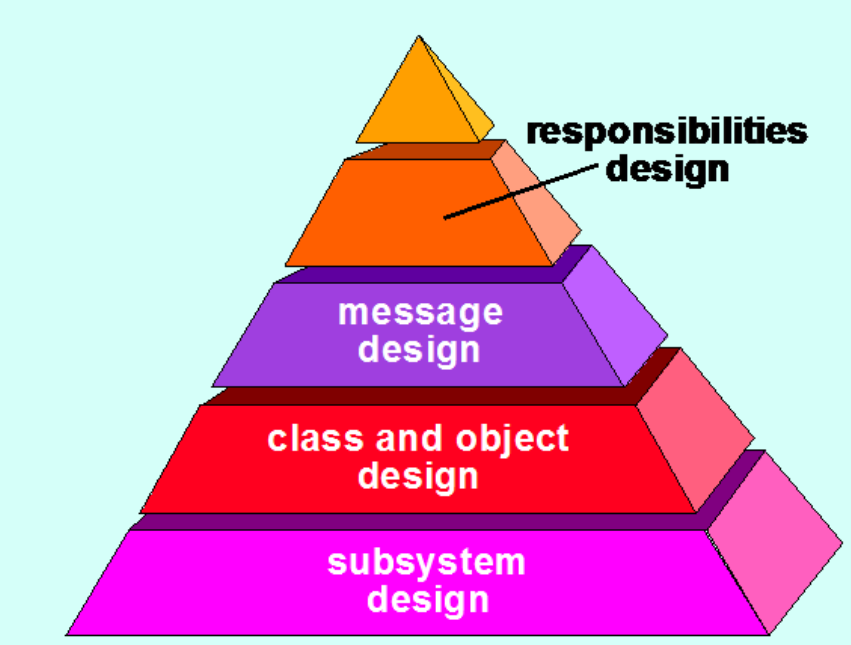
\includegraphics[width=10cm]{piramid_design.png}
\end{center}

In other words the OOD transform the "what" of OOA into the "how", adding technical details necessary for construction while preserving system correctness and maintainability

\subsection{Design Issues}
\begin{itemize}
    \item \textbf{Decomposability}: The facility with which a design method helps the designer decompose a large problem into sub-problems that are easier to solve
    \item \textbf{Composability}: the degree to which a design method ensures that program components (modules), once designed and built, can be reused to create other systems
    \item \textbf{understandability}: the ease with which a program component can be understood without reference to other information or other modules
    \item \textbf{Continuity}: the ability to make small changes in a program and have these changes manifest themselves with corresponding changes in just one or a very few modules
    \item \textbf{protection}: a architectural characteristic that will reduce the propagation of side affects if an error does occur in a given module
\end{itemize}

\subsection{The four pilars for OOD}

These are four components from the complete architecture of any well-designed OO sysyem:
\begin{itemize}
    \item \textbf{Problem domain component}:the subsystems that are
responsible for implementing customer requirements
directly
    \item \textbf{Human interaction component}:the subsystems that implement the user interface (this included reusable GUI subsystems)
    \item \textbf{Task Management Component}: the subsystems that are responsible for controlling and coordinating concurrent tasks that may be packaged within a subsystem or among different subsystems;
    \item \textbf{Data management component}: the subsystem that is responsible for the storage and retrieval of objects.
\end{itemize}

\subsection{OOA vs OOD}
\textbf{Core concept}: OOD refines the abstract OOA model into a concrete, implementable design

\begin{center}
    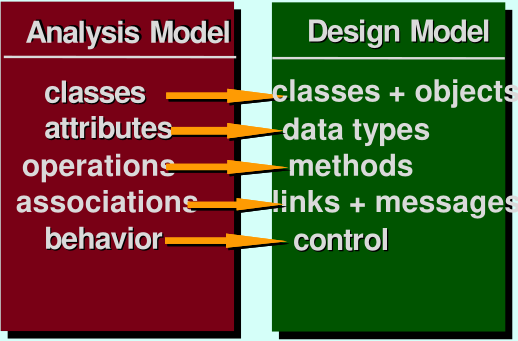
\includegraphics[width=10cm]{ship_btween_OOA_and_OOD.png}
\end{center}
what distinguishes OOD from OOA is:
\begin{itemize}
    \item LEvel of detail:
    \begin{itemize}
        \item Names are fixed
        \item Fixed signatures for messages
        \item Multiplicity \& its realization
        \item Visibility
        \item Algorithms for methods
        \item More detailed sequence/collaboration diagrams
    \end{itemize}
    \item Additional diagram notations
    
    In OOD we have class diagrams, but they refined to match the design of the sysyem.  In addition to class diagrams, we have several other diagrams:

    \begin{itemize}
        \item \textbf{Structural Diagrams}
        \item \textbf{Behavioral Diagrams}
    \end{itemize}
\end{itemize}
\subsection{Structural Diagrams for OOD in UML}
In OOD there are two Structural diagrams:
\begin{itemize}
    \item \textbf{Class Diagrams}: Their structure is the same as for OOA
    \item \textbf{Object Diagrams}:
    \begin{itemize}
        \item They deal with objects, instances of classes
        \item  They are absolutely equivalent to class diagrams
        \item  Given this, we will not analyze them in deep
    \end{itemize} 
\end{itemize}

\subsection{Behavioral Diagrams for OOD in UML}
We'll study:
\begin{itemize}
    \item \textbf{Sequence Diagrams}: Describe the interactions between objects by time ordering
    \item \textbf{Collaboration Diagrams}: Describe the interactions between the objects by organizations
\end{itemize}


\subsubsection{Human interaction component}
the subsystems that implement the user interface (this included reusable GUI subsystems);

In OOD I have class ddiagrams,but they are refined to match the design

\subsection{Statechar diagrams vs interaction diagrams}
\begin{itemize}
    \item \textbf{interaction diagrams}: show how obj interact
\end{itemize}

\subsubsection{Statechart diagrams}
First of all we'll start with a def:
\dfn{Object state}{
    We define an \textit{Object state} as the set of values that describe an object at a specific moment.  
    The state is determined based on the attribute values.
}

\begin{center}
    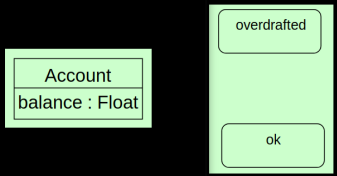
\includegraphics[width=6cm]{state.png}
\end{center}

A state can change because of an event (like the reception of a message) or can remain the same.

\begin{center}
    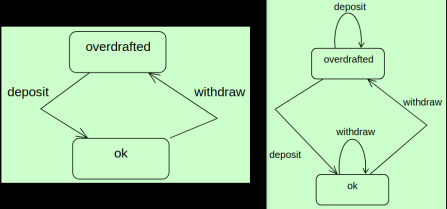
\includegraphics[width=6cm]{change_of_state.png}
\end{center}

\ex{Hockey game}{
    \begin{center}
        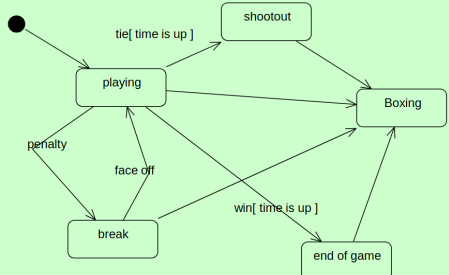
\includegraphics[width=10cm]{hockey.png}
    \end{center}
}

State diagrams are represented through rectangles with rounded borders.  
Inside them are the state variables that uniquely describe the state, and they have associated \textit{activities} or \textit{actions}.  
An activity can be long and allows interruptions, while an action happens quickly.

\begin{itemize}
    \item \textbf{entry}: an action carried out at the beginning of the state
    \item an ongoing activity carried out while in the state (e.g., showing a window)
    \item an action carried out as a response to a specific event
    \item an action carried out at the end of the state
\end{itemize}

\begin{center}
    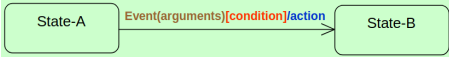
\includegraphics[width=6cm]{State-event.png}
\end{center}

Based on an event, you can decide to move from one state to another.  
The state transition is described by an arrow.

\begin{itemize}
    \item \textbf{event}: message to send
    \item \textbf{Guard condition}: the transition happens only when the guard is true.  
          The guards for the exit transitions from a state are mutually exclusive.
    \item \textbf{Action}: a process that happens rapidly and cannot be interrupted.
\end{itemize}  

\begin{center}
    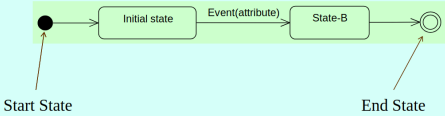
\includegraphics[width=6cm]{start-state-to-end-state.png}
\end{center}

\ex{Order Management}{
    \begin{center}
        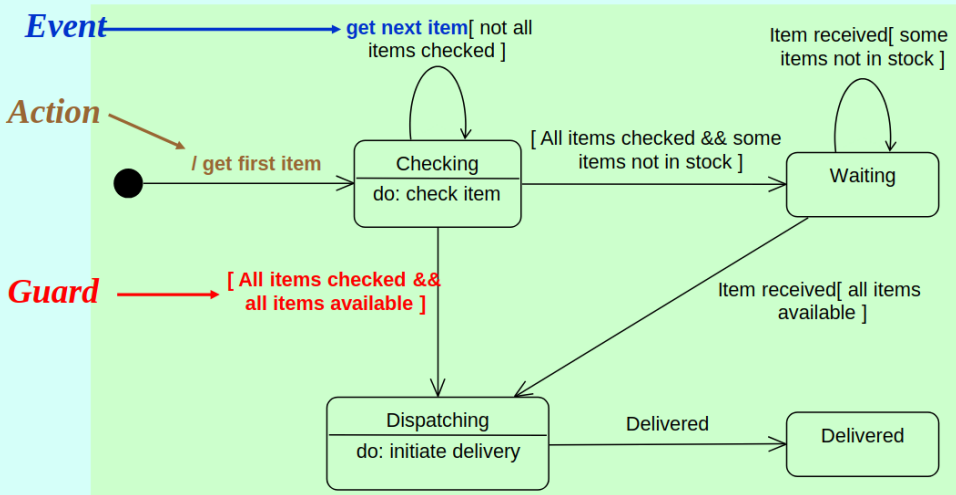
\includegraphics[width=10cm]{order_mng.png}
    \end{center}

    Now we wanna delete an order in any moment. you have two solutions:
    \begin{itemize}
        \item transitions from each state through a state "canceled"
        \item a super state and single transitions
    \end{itemize}

    Transition through "cancelled"
    \begin{center}
        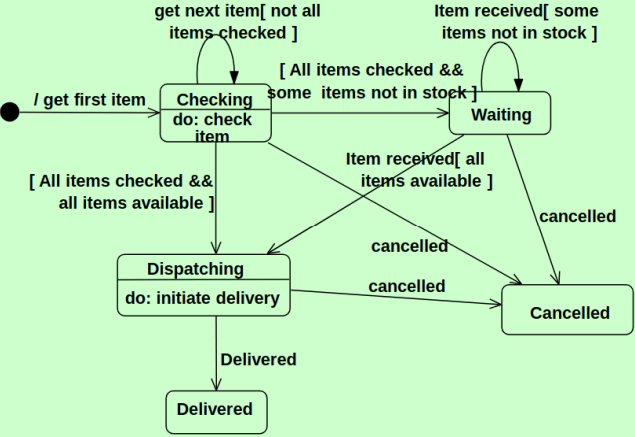
\includegraphics[width=10cm]{cancelled.png}
    \end{center}

    Super-state and sub-states
    \begin{center}
        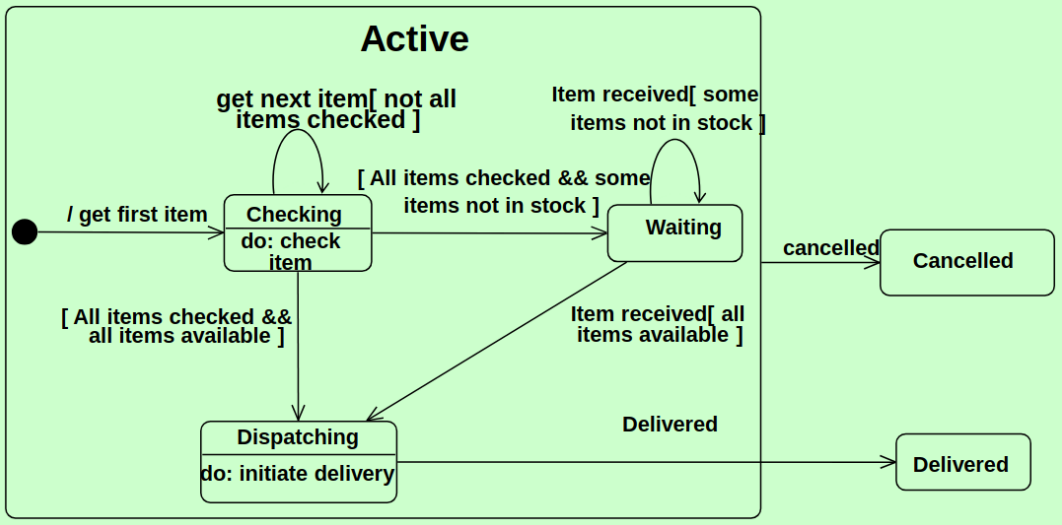
\includegraphics[width=10cm]{super-state.png}
    \end{center}
}

Statechart diagrams don't necessarily have to reference classes or objects, they can do that too refer to subsystems... In practice this is the most common way to use diagrams anyway statechart

\subsection{Activity diagrams}

\dfn{Activity Diagrams}{
    An \textit{Activity Diagram} is a behavioral diagram in UML that describes the workflow of a system, showing the flow of control from activity to activity, including support for parallel processing and decision points
}

\subsubsection{Purpose}
\begin{itemize}
    \item Model business processes
    \item Describe algorithmic workflows
    \item Show concurrent/parallel activities
    \item Document complex procedural logic
    \item Visualize use case implementations
\end{itemize}
\subsubsection{Key Characteristics}
What activity represent? Two level of abstraction:
\begin{itemize}
    \item \textbf{conceptual level}:
    \begin{itemize}
        \item Task to be done
        \item Business process step
        \item High-level action
    \end{itemize}
    \item \textbf{Specification/Implementation Level}:
    \begin{itemize}
        \item Method on a class
        \item Function execution
        \item Code block
    \end{itemize}
\end{itemize}

\ex{The coffie pot}{
    \begin{center}
        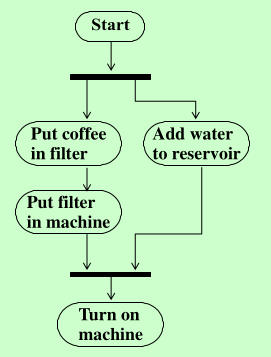
\includegraphics[width=6cm]{the_coffie_pot_basics.png}
    \end{center}
}
\subsubsection{Sync bars}
    Activities can be carried out in parallel, in any order (fork). Arrived at a bar
with multiple incoming arrows, all previous activities must be completed to continue (join).
An activity diagram shows a partial order of activities.
    \begin{itemize}
        \item \textbf{Fork (Parallel Split)} it is used for splitting into multiple concurrent flows that execute in parallel. Key points:
        \begin{itemize}
            \item One incoming edge
            \item Multiple outgoing edges
            \item All outgoing flows start simultaneously
            \item Activities execute concurrently (any order)
            \item Synchronization bar (thick line)
        \end{itemize}
        \item \textbf{Join (Parallel Merge)}, it is used for waiting all incoming parallel flows to complete before continuing. Key points:
        \begin{itemize}
            \item Multiple incoming edges
            \item One outgoing edge
            \item Synchronization point
            \item Flow continues only when ALL incoming flows complete
            \item Synchronization bar (thick line)
        \end{itemize}
    \end{itemize}

\subsubsection{conditions}
In activity diagrams we can also define "conditions": two alternative parts that you can't execute in parallel
\begin{center}
    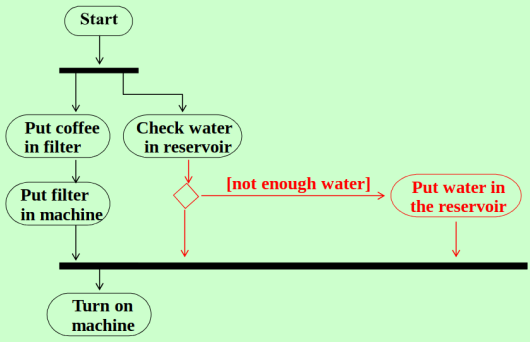
\includegraphics[width=6cm]{condition_act.png}
\end{center}

Structure:
\begin{center}
    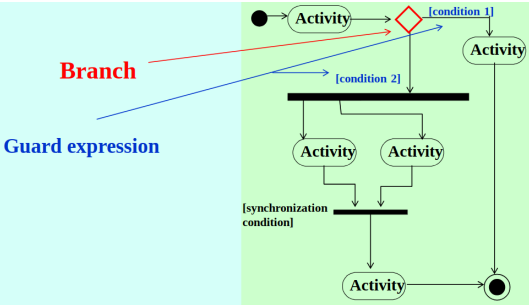
\includegraphics[width=10cm]{condition_structure.png}
\end{center}



\subsection{Interaction Diagrams}
\dfn{
    interaction Diagrams
}{
    Interaction diagrams are behavioral diagrams in UML that model the dynamic aspects of a system by showing how objects collaborate and communicate through message exchanges to accomplish specific tasks or scenarios. They emphasize the flow of control and data between objects during runtime execution
}
\subsubsection{Key charateristic}
\begin{itemize}
    \item Focus on "real" entities (Obj, not classes)
    \item Show msg e    
    \item Can represent both sync and async Communication
    \item Bridge the gap between requirements and implmentation
\end{itemize}


Interaction diagrams provide two different perspectives on the same interaction:

\subsubsection{sequence diagrams}
\begin{itemize}
    \item emphasize \textit{when} messagge are sent
    \item Shows object interactions arranged in time sequence
    \item Shows temporal ordering clearly
    \item Best for understanding flow over time
    \item Vertical timeline representation
\end{itemize}

Here we can see timelines:
\begin{center}
    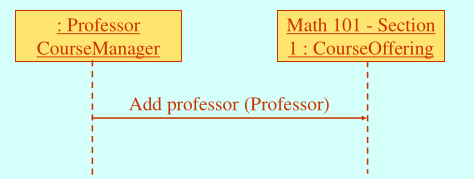
\includegraphics[width=6cm]{seq_diagram.png}
\end{center}

\ex{detailed example}{
    \begin{center}
        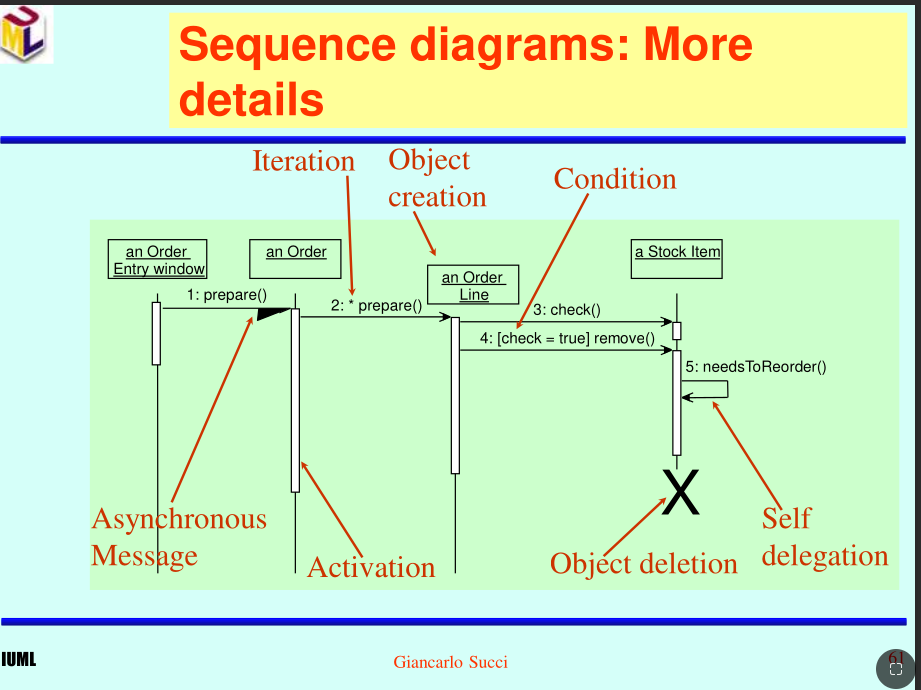
\includegraphics[width=10cm]{seq_diag_ex.png}
    \end{center}
}
\subsubsection{Content of sequence diagrams}
We have this content:
\paragraph{objects (participants)}

Lifelines:
\begin{itemize}
    \item Vertical line extending from the obj
    \item represent the obj existence time
    \item contines 'till obj is destroyed
\end{itemize}

\paragraph{Messages} There are two types of msgs:
\begin{itemize}
    \item \textbf{Sysnc msgs}:
    \begin{itemize}
        \item Full arrowhead: $ \longrightarrow $
        \item Caller wait for completion
        \item blocking operation
        \item most common in obj-oriented system
    \end{itemize}
    \item \textbf{Async msgs (signals)}:
    \begin{itemize}
        \item Half arrowhead (stick arrow): $ \rightarrow $
        \item Sender doesn't wait for completion
        \item Non-blocking operation
        \item Used for concurrent operations
    \end{itemize}
    they can do three functions:
    \begin{itemize}
        \item making a new thread
        \item making a new obj
        \item communicate with a thread already in execution
    \end{itemize}
    \item \textbf{Return Messages}:
    \begin{itemize}
        \item Typically shown as a dashed arrow: $ \dashrightarrow $
    \end{itemize}
\end{itemize}

\begin{center}
    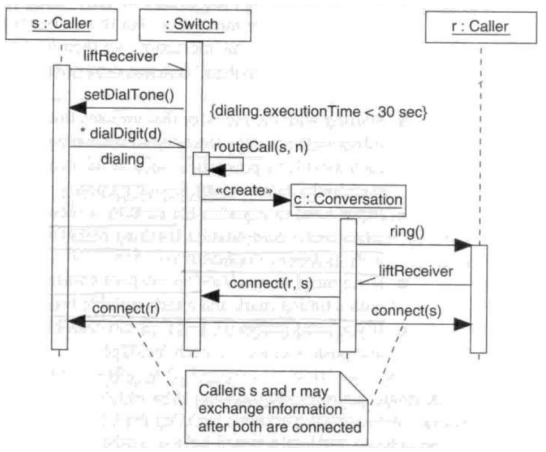
\includegraphics[width=10cm]{complete_example_of_seqdiagram.png}
\end{center}